\competentie
{% competentieformulier
	\competentieformulier
	{% toelichting
		You are sensitive, accessible and persuasive in your communications with various types of target groups, including clients. You consider the client's need your first priority, make clear arrangements and continuously check whether your performance has been satisfactory.
	}
	{% deelcompetenties
		communicating,%
		reporting,%
		customer focus%
	}
	{%
		Proof
	}
	{%
		customer focus
	}
	{% verwijzing naar bewijs
		\ref{fig:emailclient}
	}
}
{% bewijzen
	\bewijs
	{% naam
		communication with client to achieve best possible product.
	}
	{% starr
		\starr
		{% betreft
			Creating application for a client and communicating interest.
		}
		{% datum
			20-05-2022
		}
		{% situatie
			A client for which I worked for at Basenet asked me to create a product inventory.
			The client struggled to inventory their product.

			With strict ISO regulation in their sector keeping a tight inventory of products was necessary.

		}
		{% taak
			Communicate on the best flow the application should have and how it's going to be used.
			It needs to be as easy as possible to add en remove products in the application.

			The user of the application shouldn't struggle with the usage as this will decrease the experience of the customer.
		}
		{% activiteiten
			I came up with a design were the user has minimal interaction with the application.

			By listening to the wishes of the client I understood the process and the workflow of the user.
			Based on this data I created an experience were the user select their location and is able to interact with the application by pressing buttons.

		}
		{% resultaat
			By communicating with the client we achieved a exprience that is designed around the user.
		}
		{% reflectie
			The application will begin it's first round of testing soon.
			With the test I expect there to be feedback.

			The application is currently designed around a process which I understood from a talk.
			With actual usage there could be lots of improvements to be made.
		}
		{
			Hille: Hille@vaccinatiepunt.nl
		}
	}
	{% bewijs

		\begin{figure}
			\begin{center}
				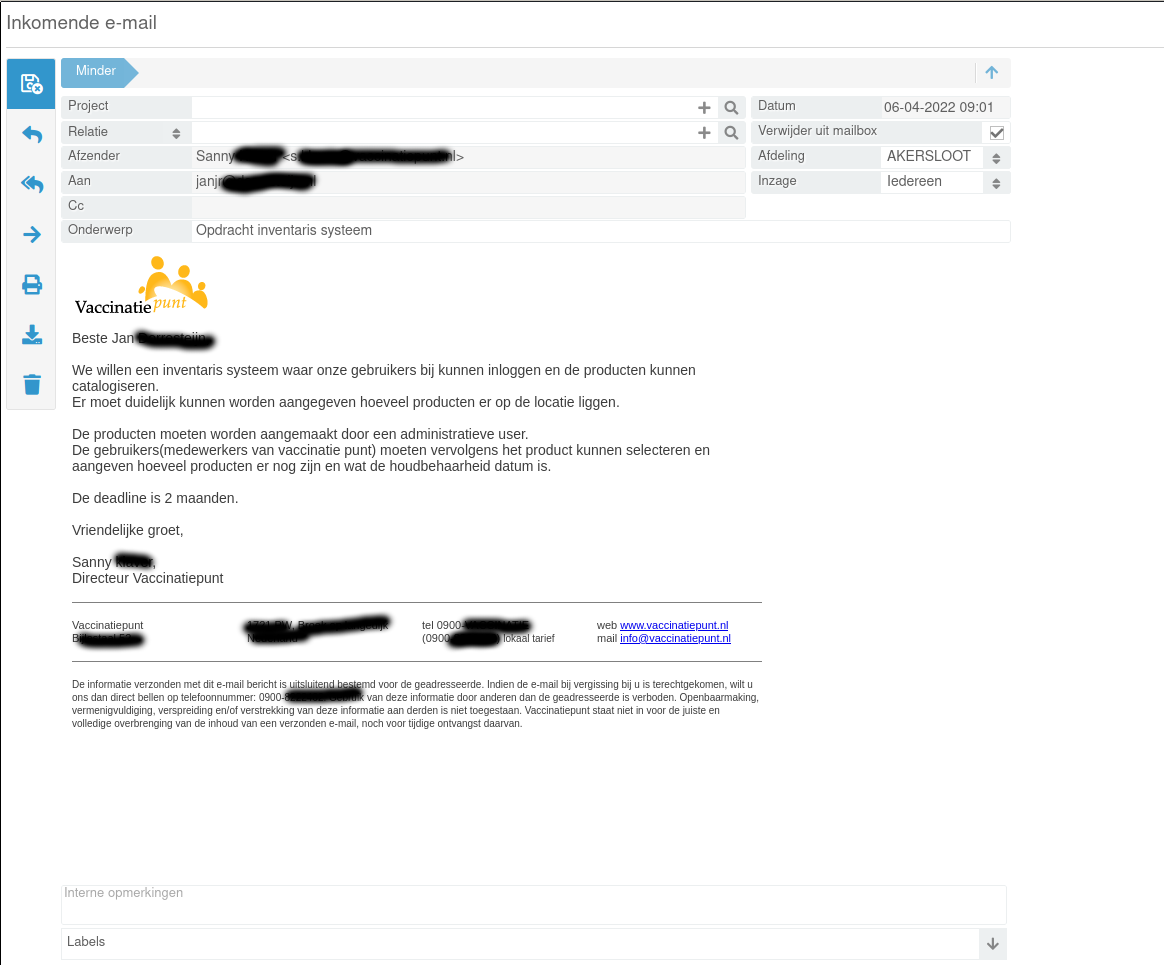
\includegraphics[width=0.95\textwidth]{images/email.png}
			\end{center}
			\caption{email client}
			\label{fig:emailclient}
		\end{figure}
	},
}
